\section{Framework Structure}
\label{sec:framework}
We now discuss Atlas' aptitude as censorship analysis platform and continue by
presenting \textsf{Cartography}, our censorship analysis framework which is
based on RIPE Atlas.

\subsection{RIPE Atlas Background}
% Some basic information about Atlas.
Having been founded in 2010 by RIPE NCC, Atlas~\cite{atlas} is a globally
distributed Internet measurement network consisting of probes run by
volunteers.  Once a user connected her probe to the network, it can be used for
measurements and the user is also able to run custom measurements by spending
some of the network's currency, Atlas credits.  These credits are awarded
automatically based on the uptime of contributed probes.  Measurements can be
run either over the web frontend, or over a HTTP-based API.

% Geographic and topological distribution.
An ideal censorship measurement platform features high geographic and
topological diversity, thereby facilitating measurements in any region where
censorship occurs.  While Atlas probes are distributed throughout the world,
there is a significant bias towards the U.S. and Europe as can be seen in
Figure~\ref{fig:probe_distribution}.  As for Atlas' topography, only 68
autonomous systems contain 40\% of all Atlas probes with the three most common
autonomous systems being 7922 (4.4\%, Comcast Cable Communications), 3320
(3.2\%, Deutsche Telekom), and 6830 (2.8\%, Liberty Global Operations).  While
not optimal, most censoring regions still contain at least several probes.

\begin{figure}[t]
\centering
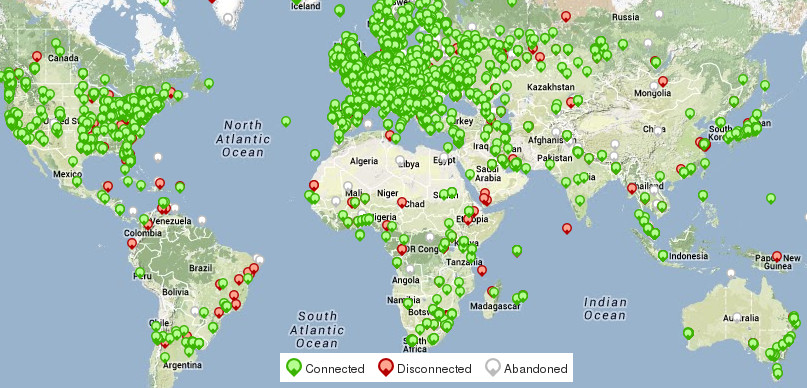
\includegraphics[width=0.48\textwidth]{diagrams/probe_distribution.jpg}
\caption{The geographic distribution of Atlas probes as of May 2014.  Green
icons represent active probes and red icons represent probes which are
currently offline.  The distribution is biased towards the U.S. and Europe.}
\label{fig:probe_distribution}
\end{figure}

% What kind of measurements does Atlas allow?
As of May 2014, Atlas allows four types of measurements; ping, traceroute, DNS
resolution, and X.509 certificate fetching.  All four measurement types can
further be parameterized for more fine-grained control.  HTTP requests are not
possible at this point due to concerns.  While Atlas clearly lacks the
flexibility of comparable platforms (see Table~\ref{tab:comparison}), it makes
up for it with comparably high diversity and its continued growth.  After all,
we do not expect Atlas to replace existing platforms such as OONI but rather to
\emph{complement} them.

% TODO - Should we talk about our crappy command-line interface?

% We also need to mention how you can stablish a big experiments using RIPE.
% And mention about the propblem of how you frist need to submit your
% experiments and then it will give you predicted cost. This way we can move to
% cost function.
As briefly mentioned above, Atlas' measurement have to be paid with so-called
credits.  The exact ``price'' of a measurement depends on the measurement type,
its parameters, and the destination(s).

\subsection{Ethical Aspects}
% The problem.
Atlas was not designed as censorship analysis platform and accordingly, its
volunteers likely do not expect that their probes will be used for such
purposes.  Careless measurements could attract a censor's attention and cause
repercussions for the respective probe operator.

% How we justify our research.
Recall that Atlas' measurement types are limited to ping, traceroute, DNS
requests and X.509 certificate fetching.  As of May 2014, it is not possible to
create HTTP requests or engage in actual, meaningful communication with
arbitrary destinations which limits the damage caused by reckless measurement.
Nevertheless, we acknowledge that care must always be taken and hope to initiate
further ethical discussions.
